% sections/02_simulations.tex -- Section 2: simulation studies S1 and S2.
% Owner: Writing Department, Task Lead 2.
% Every number in this section is produced by figures/scripts/build_sim_outputs.R from the Engineering
% per-fit records on Owls (read-only); figures/SOURCES.md lists the inputs and their sha256 sums.
% Generated pieces are \input from figures/tables/; edit the script, not the generated files.

\section{Simulation studies}\label{sec:sims}

This section compares SMC-BVS with five methods on two published simulation designs. The first design is one on
which adaptive MCMC was shown to work well; the second is a standard design for comparing selection methods across a
wide range of signal strengths. All six methods were run on the same data sets.

% ---------------------------------------------------------------------------------------------------------
\subsection{Designs}\label{sec:sims-designs}

\paragraph{Design S1.} The first design follows \citet[Sec.~4.1 and Table~1]{GriffinLatuszynskiSteel2021}, which is
adapted from \citet[Sec.~3.4.1]{YangWainwrightJordan2016}. The rows of $X$ are independent $\Normal_p(0,\Sigma)$ with
$\Sigma_{jk}=0.6^{\abs{j-k}}$, the noise variance is $\sigs^2=1$, and the first ten coefficients are nonzero,
\begin{equation}\label{eq:s1beta}
  \bstar=\mathrm{SNR}\sqrt{\log p/n}\;(2,-3,2,2,-3,3,-2,3,-2,3,0,\dots,0)^\top .
\end{equation}
We used the grid of \citet[Table~1]{GriffinLatuszynskiSteel2021}: $\mathrm{SNR}\in\{0.5,1,2,3\}$ and the four
pairs $(n,p)=(500,500)$, $(500,5000)$, $(1000,500)$ and $(1000,5000)$, 16 settings in all. \citet[Sec.~5.1]{LiangLivingstoneGriffin2022}
use the same design up to $p=50{,}000$.

\paragraph{Design S2.} The second design follows \citet[Sec.~3.1]{HastieTibshiraniTibshirani2020}. The rows of $X$ are
independent $\Normal_p(0,\Sigma)$ with $\Sigma_{jk}=\rho^{\abs{j-k}}$ and $\rho\in\{0,0.35,0.7\}$, and
$(n,p,\sz)\in\{(50,1000,5),(100,1000,10)\}$. The $\sz$ nonzero coefficients all equal one. Under beta-type~1 they sit
at equally spaced positions, $\mathrm{round}(1+(k-1)(p-1)/(\sz-1))$ for $k=1,\dots,\sz$; under beta-type~2 they are the
first $\sz$ coordinates, a block of adjacent and, for $\rho>0$, correlated predictors. The noise variance is set by
the signal-to-noise ratio, $\sigs^2=\bstar{}^\top\Sigma\bstar/\nu$, on the ten values
$\nu\in\{0.05,0.09,0.14,0.25,0.42,0.71,1.22,2.07,3.52,6\}$, equally spaced on the log scale. This gives
$2\times3\times2\times10=120$ settings.

For each of the $136$ settings we simulated $100$ data sets. Every method was fitted to the same $13{,}600$ data sets;
an MD5 checksum of each data set was compared across methods before any result was counted.

% ---------------------------------------------------------------------------------------------------------
\subsection{Methods compared}\label{sec:sims-methods}

SMC-BVS was run with its default settings (Table~\ref{tab:defaults}) and reports the median probability model
$\MPMhat$ of Section~\ref{sec:model-output}. For comparison, five methods were applied, each at the settings of its
authors.
\begin{itemize}
  \item \emph{Lasso} \citep{Tibshirani1996}, with the R package glmnet \citep{FriedmanHastieTibshirani2010} and the
  penalty chosen by tenfold cross-validation (the one-standard-error rule, the package default).
  \item \emph{SCAD} \citep{FanLi2001}, with the R package ncvreg \citep{BrehenyHuang2011}, $a=3.7$, and the penalty
  that minimises the tenfold cross-validation error.
  \item \emph{BAS} \citep{ClydeGhoshLittman2011}, the MC3 sampler of the R package BAS with its default Zellner--Siow
  prior on the coefficients and a $\BB(1,1)$ prior on the model, run for $120{,}000$ iterations after $60{,}000$ of
  burn-in.
  \item \emph{SuSiE} \citep{WangSarkarCarbonettoStephens2020}, the R package susieR with $L=20$ single effects and the
  package defaults otherwise.
  \item \emph{ASI}, the adaptive MCMC sampler of \citet{GriffinLatuszynskiSteel2021}, with their code and their settings
  for design S1: independent $\Normal(0,9)$ priors on the coefficients, a prior expected model size of $10$, and $25$
  chains of $6{,}000$ iterations, the first $2{,}000$ discarded.
\end{itemize}
For BAS, SuSiE and ASI the selected model is the median probability model, $\{j:\PIPhat_j>0.5\}$, as for SMC-BVS; for
the lasso and SCAD it is the set of nonzero coefficients. The three Bayesian competitors use priors that differ from
ours, so their posteriors differ from ours as well; the comparison is between methods as their authors run them, not
between samplers of one posterior. Each fit ran on a single core of a computing cluster with heterogeneous nodes.

% ---------------------------------------------------------------------------------------------------------
\subsection{Performance measures}\label{sec:sims-metrics}

Let $\Shat$ denote the model selected by a method for one data set and $\Sz$ the true model. We report, for each
setting, averages over the $100$ data sets of the following.
\begin{itemize}
  \item \emph{Exact recovery}: $\ind{\Shat=\Sz}$, reported as the number of data sets out of $100$.
  \item \emph{False positives} $\mathrm{FP}=\abs{\Shat\setminus\Sz}$, \emph{false negatives}
  $\mathrm{FN}=\abs{\Sz\setminus\Shat}$, and the \emph{Hamming distance} $\abs{\Shat\,\triangle\,\Sz}=\mathrm{FP}+\mathrm{FN}$.
  \item \emph{Precision} $1-\mathrm{FP}/\max(\abs{\Shat},1)$, \emph{recall} $\abs{\Shat\cap\Sz}/\sz$, and
  $F_1=2\abs{\Shat\cap\Sz}/(2\abs{\Shat\cap\Sz}+\mathrm{FP}+\mathrm{FN})$, all computed per data set and then
  averaged. An empty $\Shat$ makes no false selection and has precision one. Precision is one minus the false
  selection rate, and recall is one minus the negative selection rate, of \citet[Sec.~4.2]{SongLiang2015}.
  \item \emph{Run time}: the wall-clock time of one fit on one core, including data generation and diagnostics, and the
  CPU hours billed by the cluster scheduler for it.
\end{itemize}
Intervals for exact recovery are Wilson $95\%$ intervals \citep{Wilson1927}. A fit that failed is counted as
$\Shat=\emptyset$. This happened only for BAS in S2 (81 of 12,000 fits; numerical failures at $n=50$ and nine fits
killed for exceeding $64$\,GB of memory).

% ---------------------------------------------------------------------------------------------------------
\subsection{Results for design S1}\label{sec:sims-s1}

\begin{figure}[t]\centering
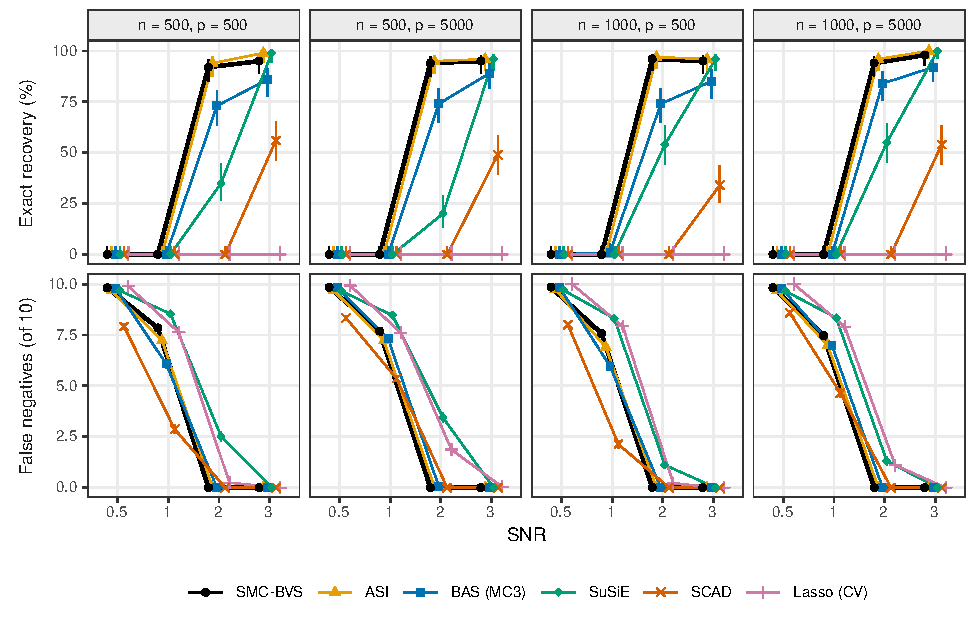
\includegraphics[width=\textwidth]{figures/fig_s1_exact}
\caption{Design S1: percentage of the $100$ data sets of each setting on which the selected model equals $\Sz$, with
Wilson $95\%$ intervals. Points are offset horizontally for legibility.}\label{fig:s1-exact}
\end{figure}

\begin{table}[t]\centering\small
\caption{Design S1: exact recovery (out of $100$ data sets per setting, $400$ in the pooled rows) at the two
strongest signals. The largest count in each row is in bold.}\label{tab:s1-exact}
% GENERATED by figures/scripts/build_sim_outputs.R -- do not edit.
\begin{tabular}{llrrrrrr}
\toprule
$(n,p)$ & SNR & SMC-BVS & ASI & BAS (MC3) & SuSiE & SCAD & Lasso (CV) \\
\midrule
$(500,500)$ & 2 & 92 & \textbf{94} & 73 & 35 & 0 & 0 \\
 & 3 & 95 & \textbf{99} & 86 & \textbf{99} & 56 & 0 \\
$(500,5000)$ & 2 & 94 & \textbf{95} & 74 & 20 & 0 & 0 \\
 & 3 & 95 & \textbf{96} & 89 & \textbf{96} & 49 & 0 \\
$(1000,500)$ & 2 & 96 & \textbf{97} & 74 & 54 & 0 & 0 \\
 & 3 & 95 & \textbf{96} & 85 & \textbf{96} & 34 & 0 \\
$(1000,5000)$ & 2 & 94 & \textbf{96} & 84 & 55 & 0 & 0 \\
 & 3 & 98 & \textbf{100} & 92 & \textbf{100} & 54 & 0 \\
\midrule
all (of 400) & 2 & 376 & \textbf{382} & 305 & 164 & 0 & 0 \\
 & 3 & 383 & \textbf{391} & 352 & \textbf{391} & 193 & 0 \\
\bottomrule
\end{tabular}

\end{table}

\begin{table}[t]\centering\small
\caption{Design S1: accuracy and cost of SMC-BVS and ASI by $(n,p)$, over the $400$ fits at all four signal
strengths. Wall times are per fit on one core; CPU hours are as billed by the cluster scheduler, which counts each
single-core job as two CPUs.}\label{tab:s1-cost}
% GENERATED by figures/scripts/build_sim_outputs.R -- do not edit.
\begin{tabular}{llrrrrrr}
\toprule
 & & & \multicolumn{3}{c}{wall time per fit} & & \\
\cmidrule(lr){4-6}
$(n,p)$ & method & exact & median & 90\% & max & CPU-h & escalated \\
\midrule
$(500,500)$ & SMC-BVS & 187 & 1.4\,min & 3.2\,min & 13.1\,min & 0.05 & 12 \\
 & ASI & 193 & 19.0\,min & 22.8\,min & 28.5\,min & 0.63 & -- \\
\addlinespace[2pt]
$(1000,500)$ & SMC-BVS & 191 & 1.2\,min & 2.6\,min & 9.4\,min & 0.04 & 16 \\
 & ASI & 193 & 20.5\,min & 25.3\,min & 29.1\,min & 0.69 & -- \\
\addlinespace[2pt]
$(500,5000)$ & SMC-BVS & 189 & 2.2\,h & 5.4\,h & 18.0\,h & 4.37 & 104 \\
 & ASI & 191 & 2.6\,h & 2.7\,h & 3.0\,h & 5.12 & -- \\
\addlinespace[2pt]
$(1000,5000)$ & SMC-BVS & 192 & 1.6\,h & 5.9\,h & 15.4\,h & 2.98 & 108 \\
 & ASI & 196 & 2.7\,h & 2.9\,h & 3.1\,h & 5.45 & -- \\
\bottomrule
\end{tabular}

\end{table}

Figure~\ref{fig:s1-exact} and Table~\ref{tab:s1-exact} show that S1 separates into two regimes. At
$\mathrm{SNR}\le1$ no method recovers $\Sz$: one success for BAS in $1{,}600$ fits, none for the others. At
$\mathrm{SNR}\ge2$, SMC-BVS recovers $\Sz$ in $92$ to $98$ of the $100$ data sets of every setting, $759$ of $800$ in
all, and the result does not depend on $(n,p)$. ASI is the strongest competitor, with $773$ of $800$. On the same data
sets the two methods differ in $16$ of $1{,}600$ fits, and ASI is the one that succeeds in $15$ of them (exact
McNemar test, $p<0.001$). The gap is therefore real but small: about one data set in a hundred at $\mathrm{SNR}\ge2$.
SuSiE matches ASI at $\mathrm{SNR}=3$ ($391$ of $400$) but drops to $164$ of $400$ at $\mathrm{SNR}=2$, where
SMC-BVS has $376$. BAS reaches $305$ and $352$ of $400$ at $\mathrm{SNR}=2$ and $3$. Of the $41$ misses of SMC-BVS
at $\mathrm{SNR}\ge2$, $37$ select a model that our posterior scores at least as high as $\Sz$, and nearly all of
them add one variable (the mean number of false positives is $0.05$ and of false negatives below $0.01$). The misses
are a property of the posterior under our prior, not of the sampler.

The two penalised methods behave differently. Cross-validated lasso never recovers $\Sz$: at $\mathrm{SNR}\ge2$ it misses fewer than one true
predictor on average but adds $36$ to $52$ false ones. SCAD adds fewer, and recovers $\Sz$ in
$193$ of $400$ data sets at $\mathrm{SNR}=3$, but none at $\mathrm{SNR}=2$. Over all of S1 the lasso and SCAD select
$22.2$ and $23.2$ false positives per fit, against $0.03$ for SMC-BVS and ASI.

At weak signal the methods differ in what they miss. At $\mathrm{SNR}=1$, SMC-BVS selects almost nothing that is
false ($0.01$ false positives per fit) and misses $7.65$ of the ten true predictors; ASI misses $7.08$ and BAS
$6.59$. ASI has the smaller Hamming distance in $185$ of the $800$ fits at $\mathrm{SNR}\le1$, against $8$ for
SMC-BVS. SMC-BVS is the more conservative of the two when the signal is weak.

Table~\ref{tab:s1-cost} sets accuracy against cost. At $p=500$ a fit of SMC-BVS takes a median of $1.2$ minutes on
one core and ASI $20.0$ minutes, and SMC-BVS costs $0.04$--$0.05$ billed CPU hours per fit against $0.63$--$0.69$
for ASI. At $p=5000$ the medians are closer, $1.8$ hours against $2.6$ hours, and SMC-BVS has the longer tail: its
$90\%$ quantile is $5.5$ hours and its slowest fit took $18.0$ hours, whereas no ASI fit took more than $3.1$ hours.
ASI runs a fixed number of iterations, while SMC-BVS adapts its temperature schedule to the data
(Section~\ref{sec:model-sampler}), so its cost varies from one data set to the next. Over all $1{,}600$ fits SMC-BVS
was billed $4{,}110$ CPU hours and ASI $4{,}703$; the former includes ten first attempts that hit the $24$-hour limit
and were rerun.
% ---------------------------------------------------------------------------------------------------------
\subsection{Results for design S2}\label{sec:sims-s2}

\begin{figure}[t]\centering
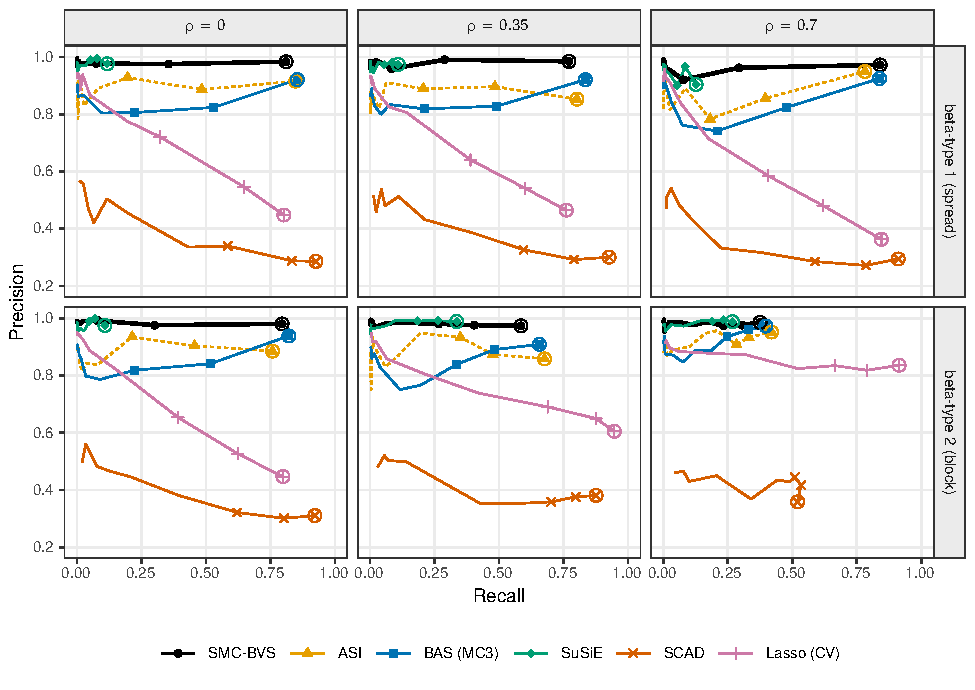
\includegraphics[width=\textwidth]{figures/fig_s2_pr}
\caption{Design S2: mean precision against mean recall as the signal-to-noise ratio $\nu$ increases from $0.05$
to $6$, pooled over $n\in\{50,100\}$ ($1{,}200$ fits per point except ASI). Filled points mark $\nu=2.07$, $3.52$
and $6$, and the circled point is $\nu=6$. ASI (dashed) is interim: $25$ data sets per setting ($300$ fits per
point).}\label{fig:s2-pr}
\end{figure}

\begin{table}[t]\centering\small
\caption{Design S2 at the three strongest signals, by beta-type, pooled over $n$ and $\rho$: exact recovery
(percentage of $600$ data sets), mean precision and mean recall. $^\dagger$ASI is interim: the first $25$ data sets
of each setting ($150$ per cell).}\label{tab:s2-main}
% GENERATED by figures/scripts/build_sim_outputs.R -- do not edit.
\begin{tabular}{ll*{5}{r}c*{5}{r}}
\toprule
 & & \multicolumn{5}{c}{beta-type 1 (spread support)} & & \multicolumn{5}{c}{beta-type 2 (block support)} \\
\cmidrule{3-7}\cmidrule{9-13}
$\nu$ & method & exact & $\abs{\Shat}$ & empty & prec. & recall & & exact & $\abs{\Shat}$ & empty & prec. & recall \\
\midrule
2.07 & SMC-BVS & 0 & 0.6 & 63 & 0.87 & 0.08 & & 0 & 1.5 & 26 & 0.98 & 0.19 \\
 & ASI & 1 & 1.5 & 31 & 0.82 & 0.18 & & 1 & 2.2 & 12 & 0.90 & 0.27 \\
 & BAS (MC3) & 1 & 3.1 & 35 & 0.67 & 0.21 & & 1 & 3.0 & 15 & 0.84 & 0.27 \\
 & SuSiE & 0 & 0.4 & 62 & 0.88 & 0.05 & & 0 & 1.1 & 29 & 0.99 & 0.14 \\
 & SCAD & 0 & 19.4 & 8 & 0.26 & 0.59 & & 0 & 17.5 & 3 & 0.36 & 0.61 \\
 & Lasso (CV) & 0 & 9.1 & 33 & 0.48 & 0.37 & & 2 & 9.0 & 13 & 0.69 & 0.58 \\
\addlinespace[3pt]
3.52 & SMC-BVS & 10 & 2.4 & 36 & 0.96 & 0.31 & & 4 & 2.7 & 14 & 0.97 & 0.34 \\
 & ASI & 10 & 3.7 & 13 & 0.86 & 0.45 & & 5 & 3.5 & 5 & 0.91 & 0.43 \\
 & BAS (MC3) & 11 & 5.6 & 17 & 0.79 & 0.50 & & 4 & 4.2 & 7 & 0.89 & 0.44 \\
 & SuSiE & 0 & 0.6 & 51 & 0.96 & 0.08 & & 0 & 1.4 & 22 & 0.99 & 0.19 \\
 & SCAD & 0 & 24.2 & 2 & 0.27 & 0.80 & & 1 & 19.9 & 1 & 0.36 & 0.71 \\
 & Lasso (CV) & 0 & 15.4 & 17 & 0.42 & 0.62 & & 3 & 11.9 & 6 & 0.64 & 0.76 \\
\addlinespace[3pt]
6 & SMC-BVS & 64 & 6.3 & 10 & 0.98 & 0.81 & & 23 & 4.5 & 4 & 0.98 & 0.59 \\
 & ASI & 53 & 6.6 & 5 & 0.91 & 0.81 & & 19 & 5.2 & 1 & 0.91 & 0.64 \\
 & BAS (MC3) & 55 & 7.2 & 7 & 0.92 & 0.84 & & 21 & 5.3 & 3 & 0.94 & 0.63 \\
 & SuSiE & 0 & 1.0 & 40 & 0.92 & 0.12 & & 0 & 1.9 & 17 & 0.98 & 0.24 \\
 & SCAD & 0 & 25.6 & 1 & 0.29 & 0.92 & & 2 & 21.8 & 1 & 0.35 & 0.77 \\
 & Lasso (CV) & 0 & 20.9 & 8 & 0.37 & 0.80 & & 10 & 14.1 & 4 & 0.62 & 0.89 \\
\bottomrule
\end{tabular}

\end{table}

Design S2 is harder: $n/\sz=10$, and seven of its ten signal levels are too weak for any method to recover $\Sz$. For
$\nu\le1.22$ no method recovers $\Sz$ in more than one of $1{,}200$ fits per level. What separates the methods there
is what they select when the data say little. Over the $4{,}800$ fits per method at $\nu\le0.25$, SMC-BVS selects
$0.02$ false positives per fit and at most $3$ in any fit. SCAD selects $5.90$ on average and up to $43$; the lasso
$0.77$, up to $58$; BAS $0.44$, up to $39$.

The comparison is decided at $\nu\ge3.52$ (Table~\ref{tab:s2-main}, Figure~\ref{fig:s2-pr}). At $\nu=6$, SMC-BVS
recovers $\Sz$ in $523$ of $1{,}200$ data sets, BAS in $455$, the lasso in $64$, SCAD in $14$ and SuSiE in $3$. On the
first $25$ data sets of each setting, where ASI has finished, SMC-BVS recovers $\Sz$ in $130$ of $300$ and ASI in $98$;
paired on the same data sets, SMC-BVS alone succeeds in $36$ and ASI alone in $4$. At $\nu=3.52$ the order reverses:
BAS recovers $92$ of $1{,}200$ against $81$ for SMC-BVS, and ASI $27$ of $300$ against $23$. SMC-BVS keeps a
precision between $0.97$ and $0.98$ at every signal level; only SuSiE, which selects very little, is as precise. The price is recall. At
$\nu=3.52$ it finds $32\%$ of the true predictors, against $44\%$ for ASI, $47\%$ for BAS and $69\%$ for the lasso; at
$\nu=6$, $70\%$ against $71\%$, $73\%$ and $84\%$. The lasso and SCAD reach their higher recall by selecting $11$ and
$17$ false predictors per fit at $\nu=6$.

The weakest case for SMC-BVS is beta-type~2 with correlated predictors, where the true model is a block of $\sz$
adjacent columns with equal coefficients. At $\nu=6$ SMC-BVS recovers the block in $4\%$ of the data sets at
$\rho=0.35$ and in none at $\rho=0.7$, and its recall falls to $0.58$ and $0.38$. ASI (interim) and BAS fail in the same way
($0$--$6\%$ exact, recall $0.40$--$0.68$), while the lasso, which over-selects by construction, recovers the block in
$22.5\%$ of the data sets at $\rho=0.7$. The failures come from the posterior, not from the search: in $3{,}988$ of
the $3{,}992$ beta-type~2 fits with $\rho>0$ that missed $\Sz$, our posterior scores the selected model at least as
high as $\Sz$, and in none of the $4{,}000$ is the selected model larger than $\Sz$. With equal
effects on adjacent correlated columns the response depends mostly on the sum of the block, a few members of the
block reproduce that fit almost as well, and under a model prior that is sparse at $p=1000$ each further member costs
more prior mass than it adds in likelihood. The posterior then spreads over many subsets of the block: at $\nu=6$ the average
inclusion probability of a block member is between $0.39$ and $0.61$, depending on $n$ and $\rho$, and the median
probability model keeps only some of the members. In the same
settings with spread-out support (beta-type~1) SMC-BVS recovers $\Sz$ in $67.5\%$ of the data sets at $\rho=0.7$.

SuSiE recovers $\Sz$ in only $3$ of the $12{,}000$ S2 data sets. At $n/\sz\le10$ with equal moderate effects its
fitting algorithm, started at its default residual variance, stops at a local optimum with one to three active effects.
In a check on two settings, a start from the true residual variance reached a higher evidence lower bound in $31$ of
$40$ data sets. We
report SuSiE at its defaults, as for the other methods. In design S2 a fit of SMC-BVS took a median of $4.0$ minutes
($5.9$ at $n=50$, $1.2$ at $n=100$), against $30.5$ minutes for ASI (on its first $25$ data sets per setting).
